% ss_howto.tex

% How to play
\subsection{How to play}
\label{sec:howtoplay}
\textbf{Shuffle-Spires} is a turn-based game, wherein a turn has four independent steps in a strict order:
\begin{enumerate}[noitemsep]
	\item Progression
	\item Draw
	\item Attack
	\item Shuffle
\end{enumerate}
These phases are elaborated upon below.
Turn-progression is clockwize.

% Progression-phase
\subsubsection{Progression-phase}
\label{sec:playingshufflespires_progressionphase}
If you’re the current \textit{Thin-Things-Thin}; move all attacking Henchmen one step forward (\textit{Zone 1} to \textit{Zone 2} etc.)
When the previous owner of this title is slain; the title of \textit{Thin-Things-Thin} is simply given unto the next player.

Select a rule for the Progression-phase:

\paragraph{Rule $1$}
If a Henchman has reached \textit{Zone $3$}. Destroy one of the adjacent bottom Spire-sections.
If there are two adjacent Spires: flip a coin or roll the die ($1$-$5$ meaning Left card, $6$-$9$ meaning Right card).
This card is destroyed and \textit{removed from game}.

\paragraph{Rule $2$}
As with \textit{Rule $1$}, only a Spire-Section isn’t destroyed when a Henchman reaches \textit{Zone $3$}, but instead when a Henchmen is to progress from \textit{Zone $3$} to the arbitrary \textit{Zone $4$}.
This results in slightly longer gameplay.\\

\noindent
When a lower card is destroyed; the upper cards descend into the lower levels of the Spires.

% Draw-phase
\subsubsection{Draw-phase}
\label{sec:playingshufflespires_drawphase}
Draw a card from the Deck.
This card will belong to one of the suits and be numbered one through ten.
This may be seen as an attacking Henchman.

The player is to place the card in \textit{Zone $1$}, either left or right, of the Spire of the corresponding suit (that is; around the Spire in which the King of that suit is in, at the moment).

Ex. $7$ of Hearts is placed either left or right of the Spire in which the King of Hearts currently resides.

Ex. $3$ of Clubs is placed either left or right of the Spire in which the King of Clubs currently resides.

\paragraph{Optional rule}
The Ace cards are no Henchmen, and instead acts as a free shuffle.
If a Player draws an Ace-card, of any suit, that player may choose to re-arrange his Spire (meaning the spire in which his King resides) according to one of the alternatives on the \textit{Shuffle-Table}.

% fig:draw
\begin{figure}[h!]
	\centering
	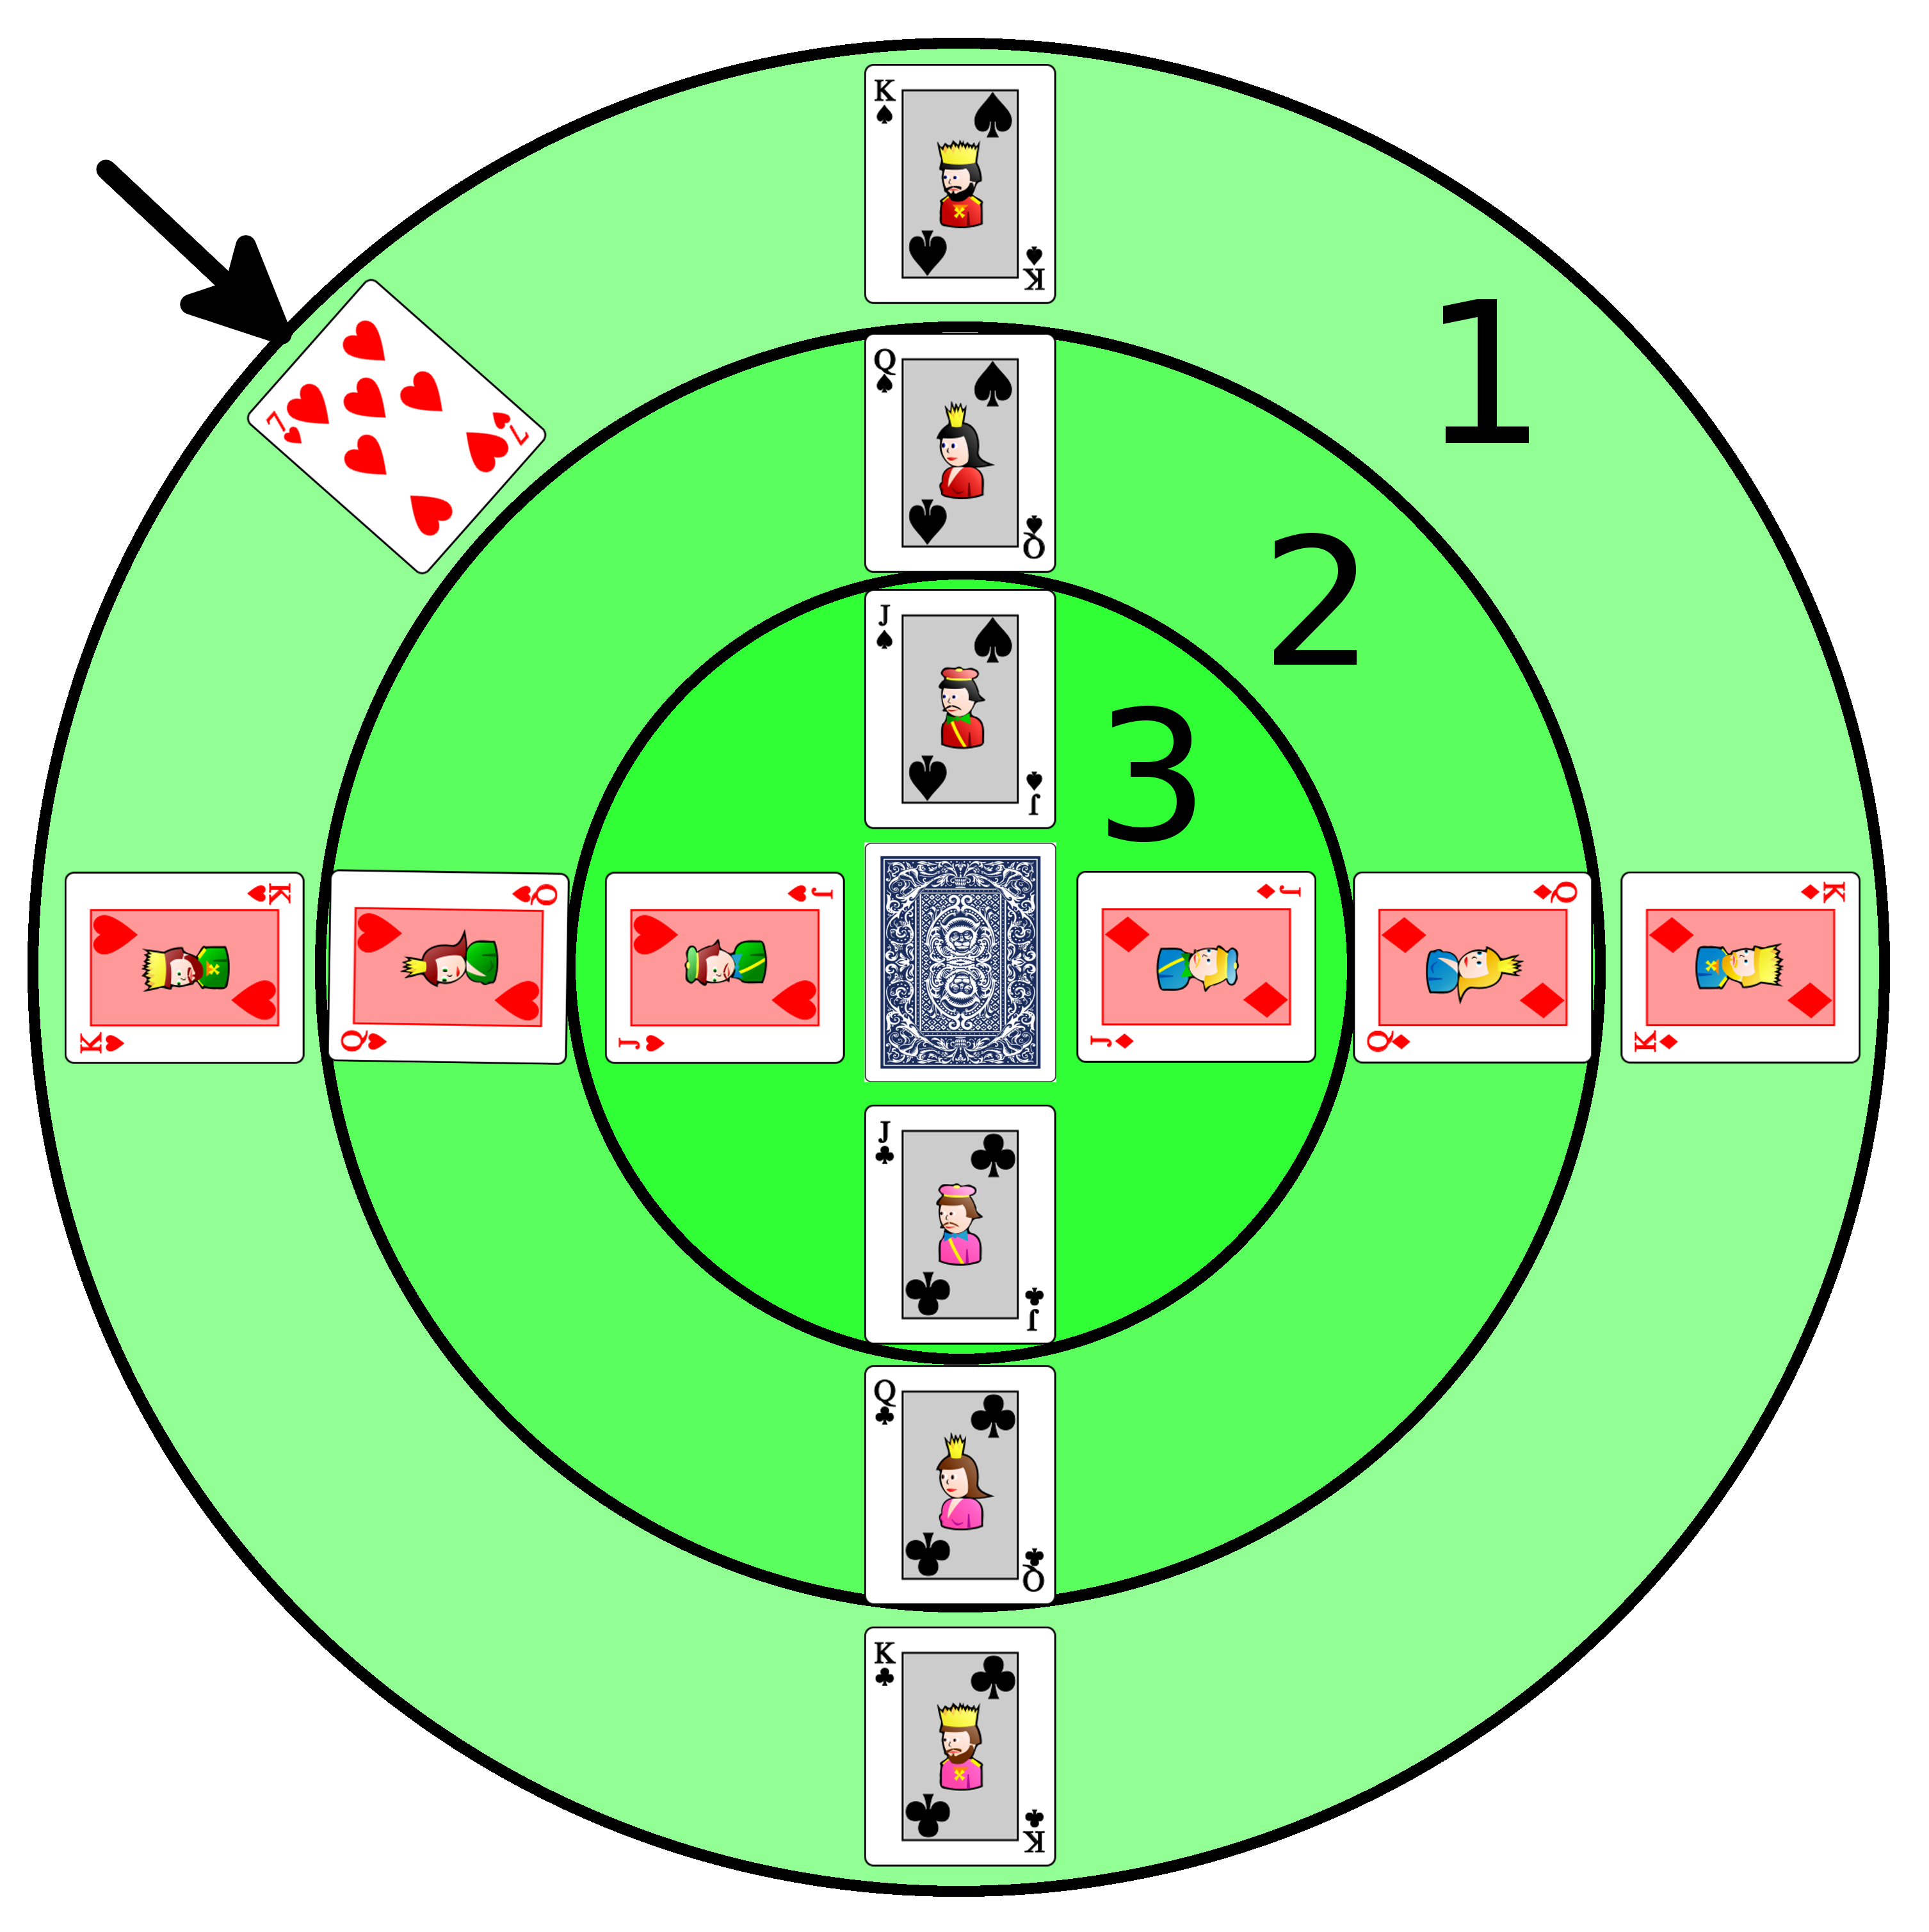
\includegraphics[width=\linewidth]{img/draw.png}
	\caption{Player Hearts draws $7$ of Hearts and places it left of the Spire in which the King of Hearts resides.}
	\label{fig:draw}
\end{figure}

% Attack-phase
\subsubsection{Attack-phase}
\label{sec:playingshufflespires_attackphase}
Each section of a Player's Spire (that is; his/her King, Queen and Jack) can attack one attacking Henchman per turn.
However, the Henchman the Player wishes to attack must be in a corresponding \textit{Zone} in relation to the attacker Spire-Section.

E.g. if King of Hearts is at the top of a Spire, in \textit{Zone $1$}, King of Hearts may attack any attacking Henchman in \textit{Zone $1$}.

E.g. if Jack of Diamonds is in the middle of a Spire, in \textit{Zone $2$}, Jack of Diamonds may attack any attacking Henchman in \textit{Zone $2$}.

Example (see Figure \ref{fig:attack}):

Player Hearts may attack card $7$ of Hearts or $9$ of Spades with King of Hearts.

Player Hearts may attack card $5$ of Hearts, $2$ of Diamonds or $4$ of Clubs with Queen of Hearts.

If Progression-Rule $1$ is used; the bottom cards will never have a chance to attack any Henchmen, and will only act as Shields.

If Progression-Rule $2$ is used; the bottom cards can attack Henchmen in \textit{Zone $3$}.

Each Spire-Section may attack only once per turn. A player may choose not to attack anything if he/she so wishes.

% fig:attack
\begin{figure}[h!]
	\centering
	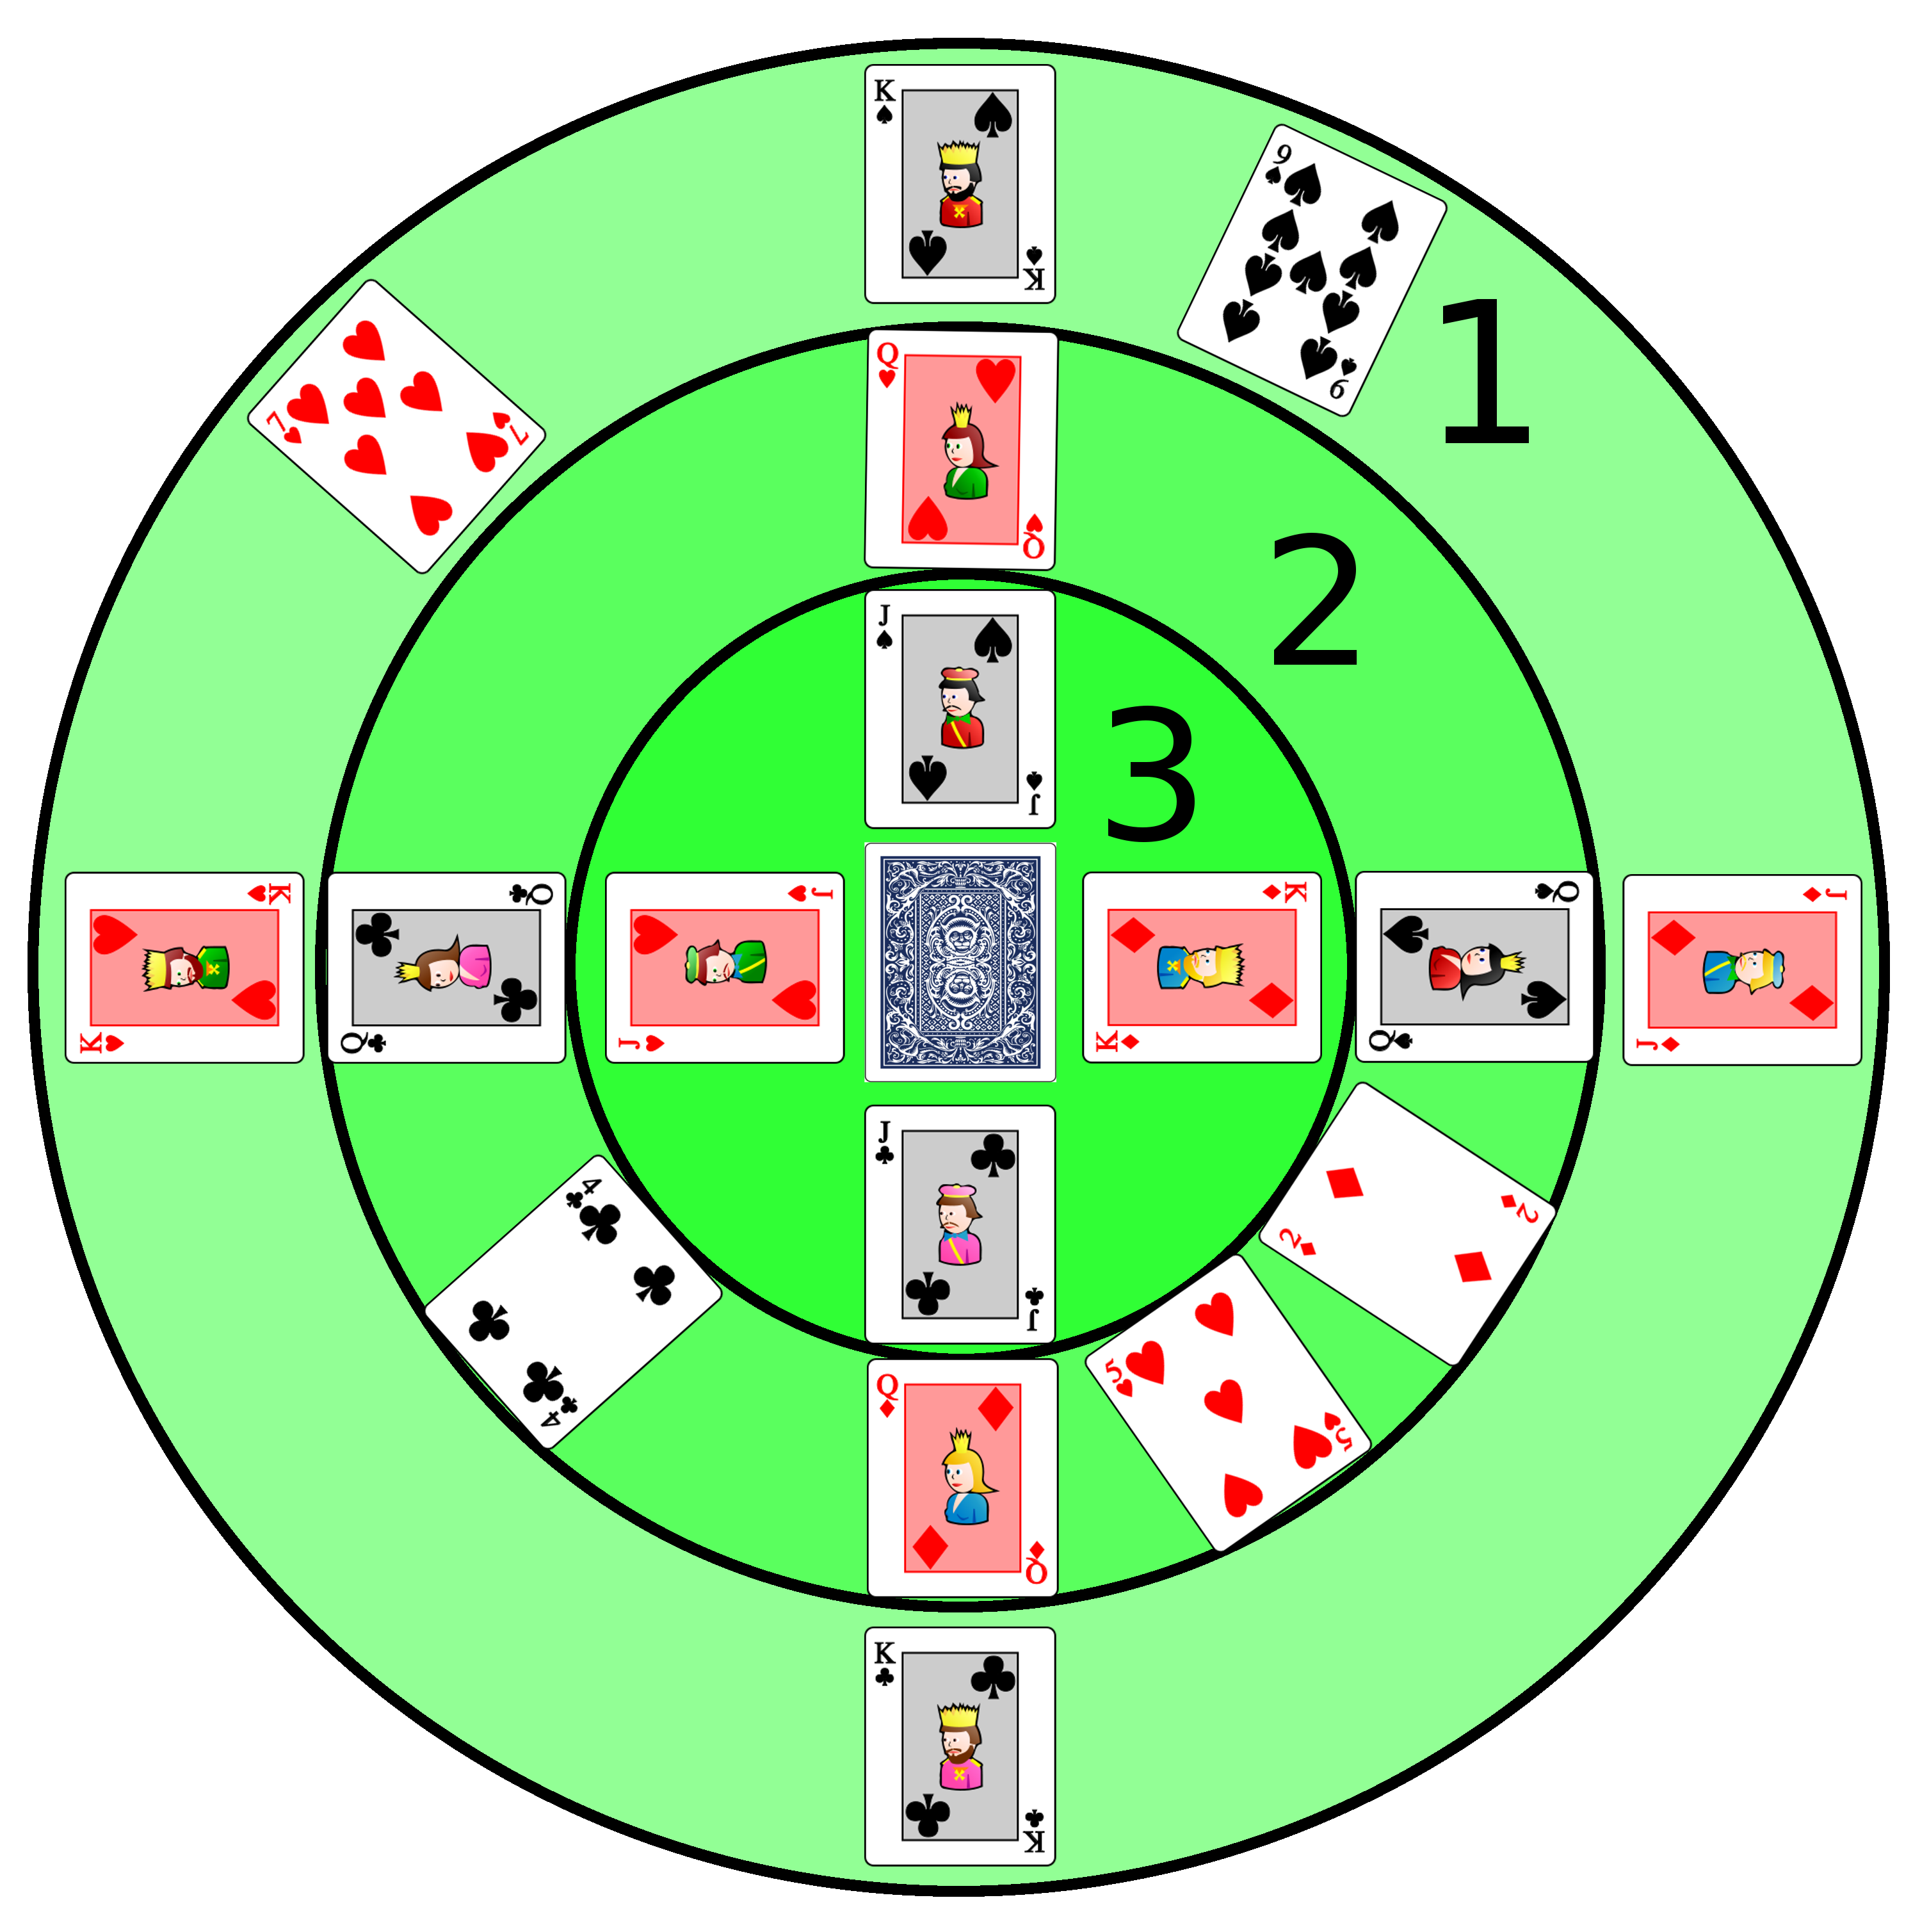
\includegraphics[width=\linewidth]{img/attack.png}
	\caption{A potential Attack-phase after a couple of turns.}
	\label{fig:attack}
\end{figure}

When a Player has chosen which Henchmen to attack - or which Henchmen not to attack - he/she will, for each attempted attack, roll the die to see whether or not the attack was sucessful.
Since the Realm of Thin-Things spawns a great deal of very thin-things indeed, some of the Kings' Henchmen are very thin, and thin-things are hard to hit.

The Henchmen are numbered one through ten (two through ten, if you're playing with the Optional Rule described under \nameref{sec:playingshufflespires_drawphase}) where smaller numbers describe thin-ness.

A player will have to roll either equal to-/or below the Henchmen's thin-ness in order to slay them.
If a player has rolled above a certain Henchman's thin-ness the attack was un-sucessful and the Henchman stays on the board.

If the attack was sucessful, the Henchman is discarded.

% Shuffle-phase
\subsubsection{Shuffle-phase}
\label{sec:playingshufflespires_shufflephase}
Each turn is ended with a roll on the \textit{Shuffle-Table} to decide how the Shuffling Spires shuffle during the Shuffle-phase.
The \textit{Shuffle-Table} is described as follows:

\begin{tabular}{ l l }
	1 & Bottom Section Right \\
	2 & Bottom Section Left \\
	3 & Middle Section Right \\
	4 & Middle Section Left \\
	5 & Top Section Right \\
	6 & Top Section Left \\
	7 & Shuffle Spire Downwards\\
	8 & Shuffle Spire Upwards \\
	9 &  Roll \textit{Shuffle-Table} twice\\
	10 & - \\
\end{tabular}

% fig:shuffle
\begin{figure}[h!]
	\centering
	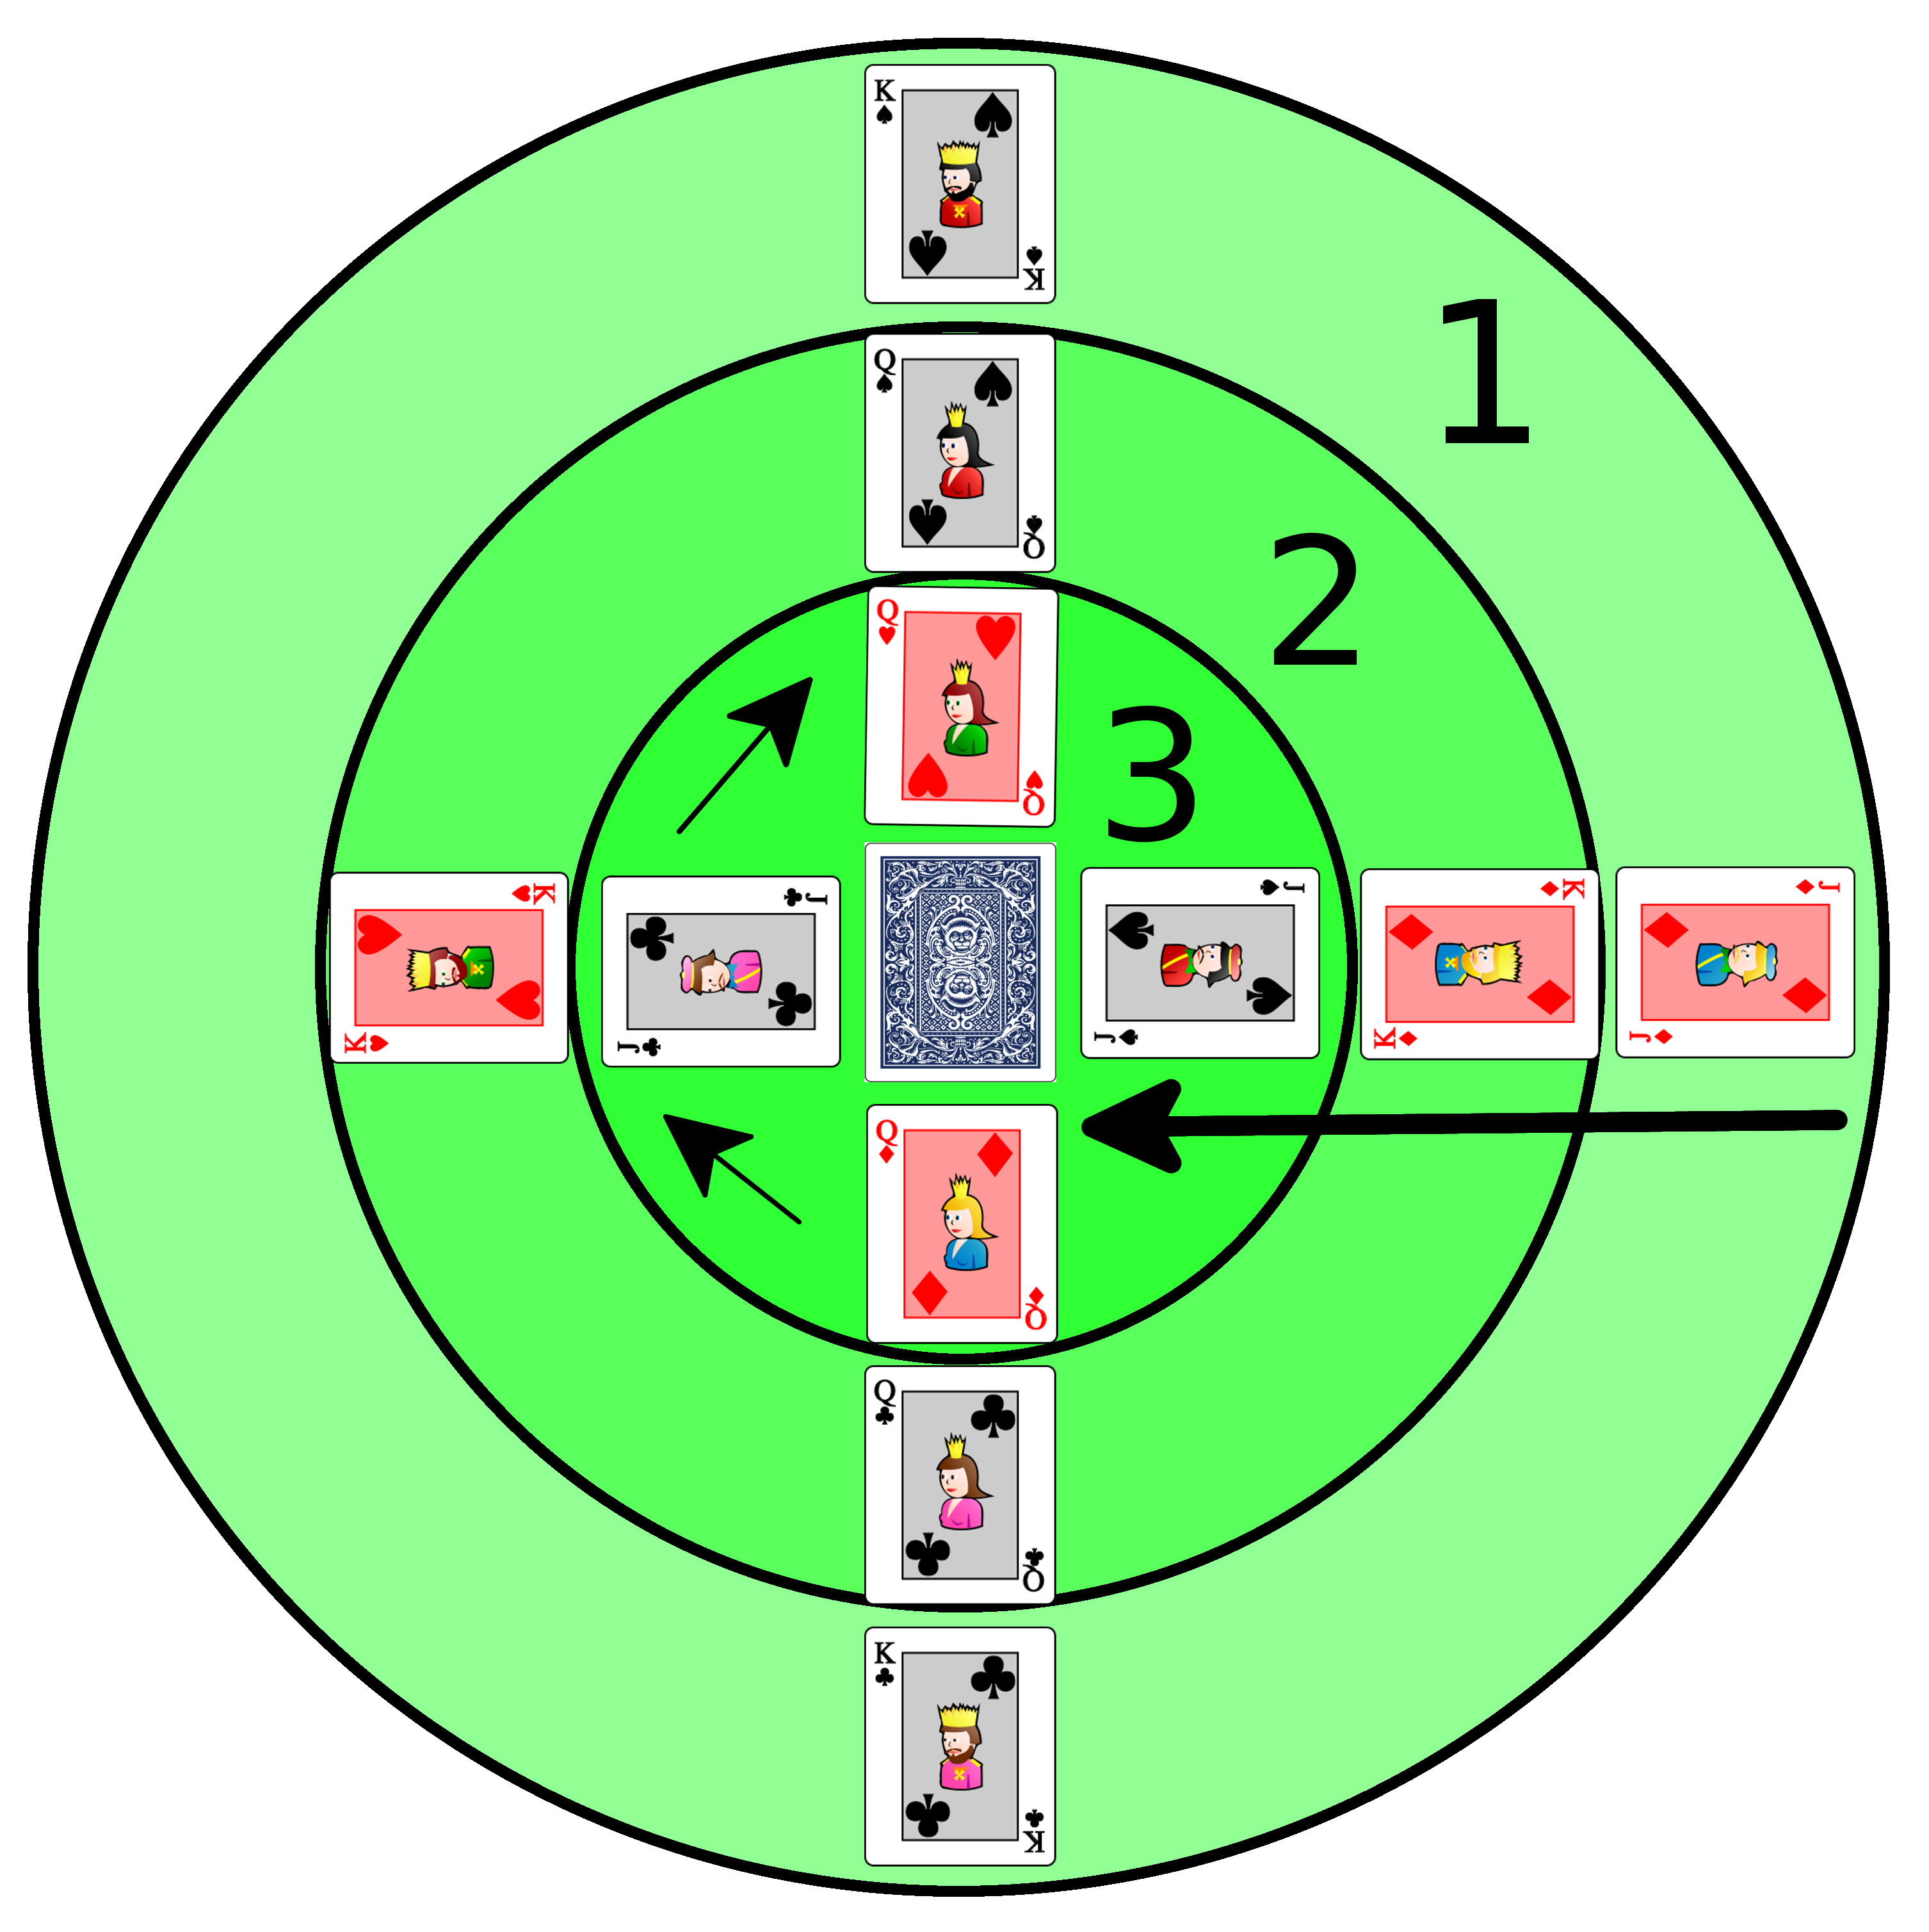
\includegraphics[width=\linewidth]{img/shuffle.png}
	\caption{Player Diamonds rolls a $9$, followed by $7$ and $2$, on the \textit{Shuffle-Table}.}
	\label{fig:shuffle}
\end{figure}

\paragraph{Notes}
If another Spire-Section occupies your Shuffled Spire-Section's new position, then relocate that Spire-Section in accordance to the \textit{Shuffle} in question.

E.g. if all bottom \textit{Zones} on the board are occupied, and a player rolls $1$ on the \textit{Shuffle-Table}, then move all bottom cards to the Right.

If your newly moved Spire-Section isn't resting steadily on lower section, then lower it.
These are very thin wind-swept Spires, not flying ones!
